\section{Exercise 1 - EdgeImpulse} %Introduction
To complete the first exercise, I decided to classify the same items used in the provided demo.
In particular, I took 20 pictures of a coin, 20 pictures of a pen and 20 pictures of the background.\bigskip

After the training with an 80/20 split, I obtained the following results:

\begin{figure}[h!]
    \centering
    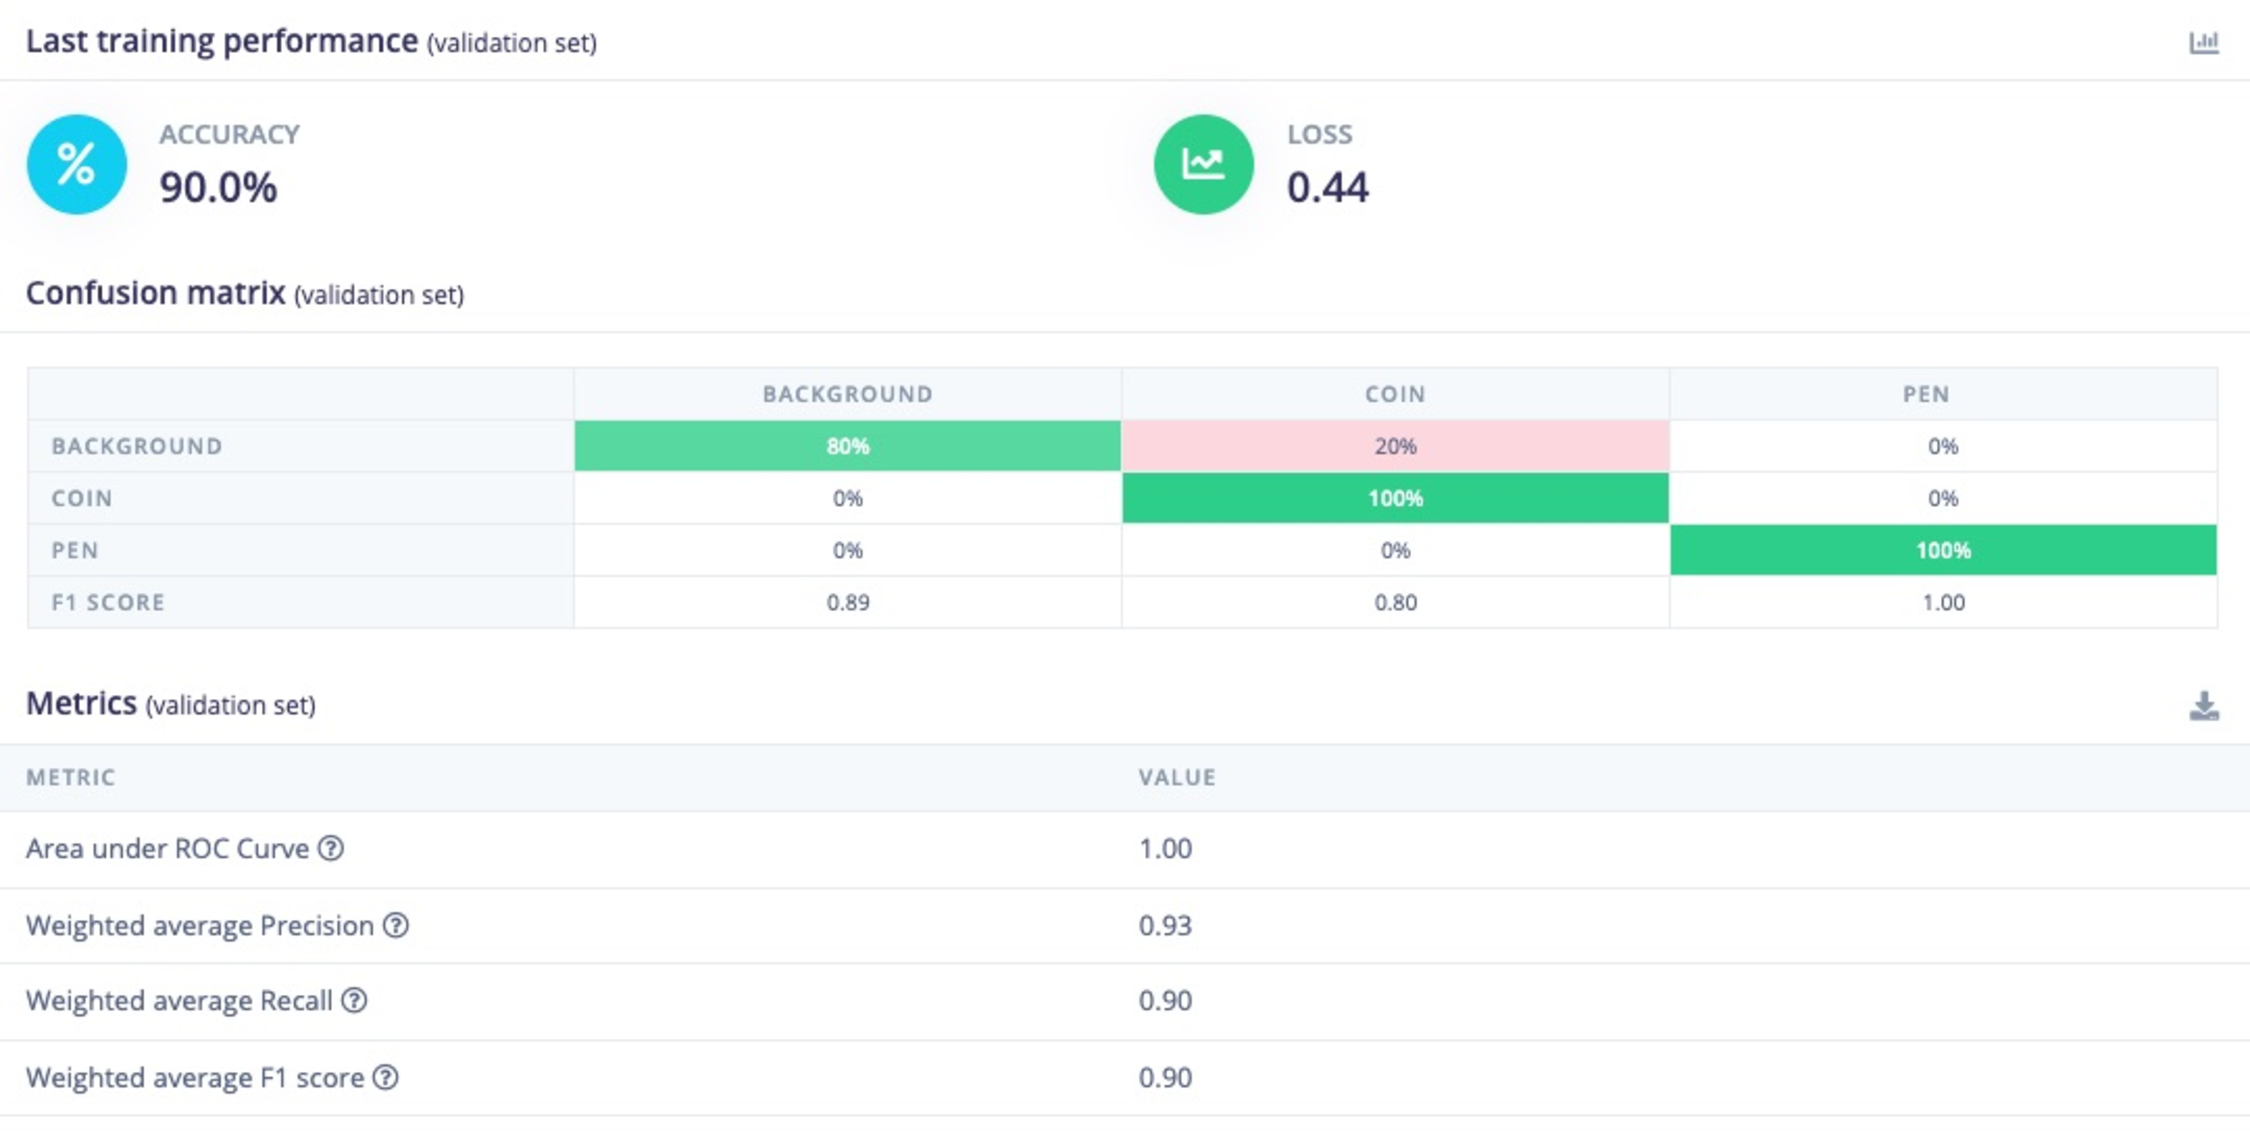
\includegraphics[width=0.8\linewidth]{Resources/Training_results.pdf} % <-- replace with your filename
    \caption{Training results}
\end{figure}

I also tested the model on the validation set, achieving an accuracy of 100\% as shown in the following screenshot:

\begin{figure}[h!]
    \centering
    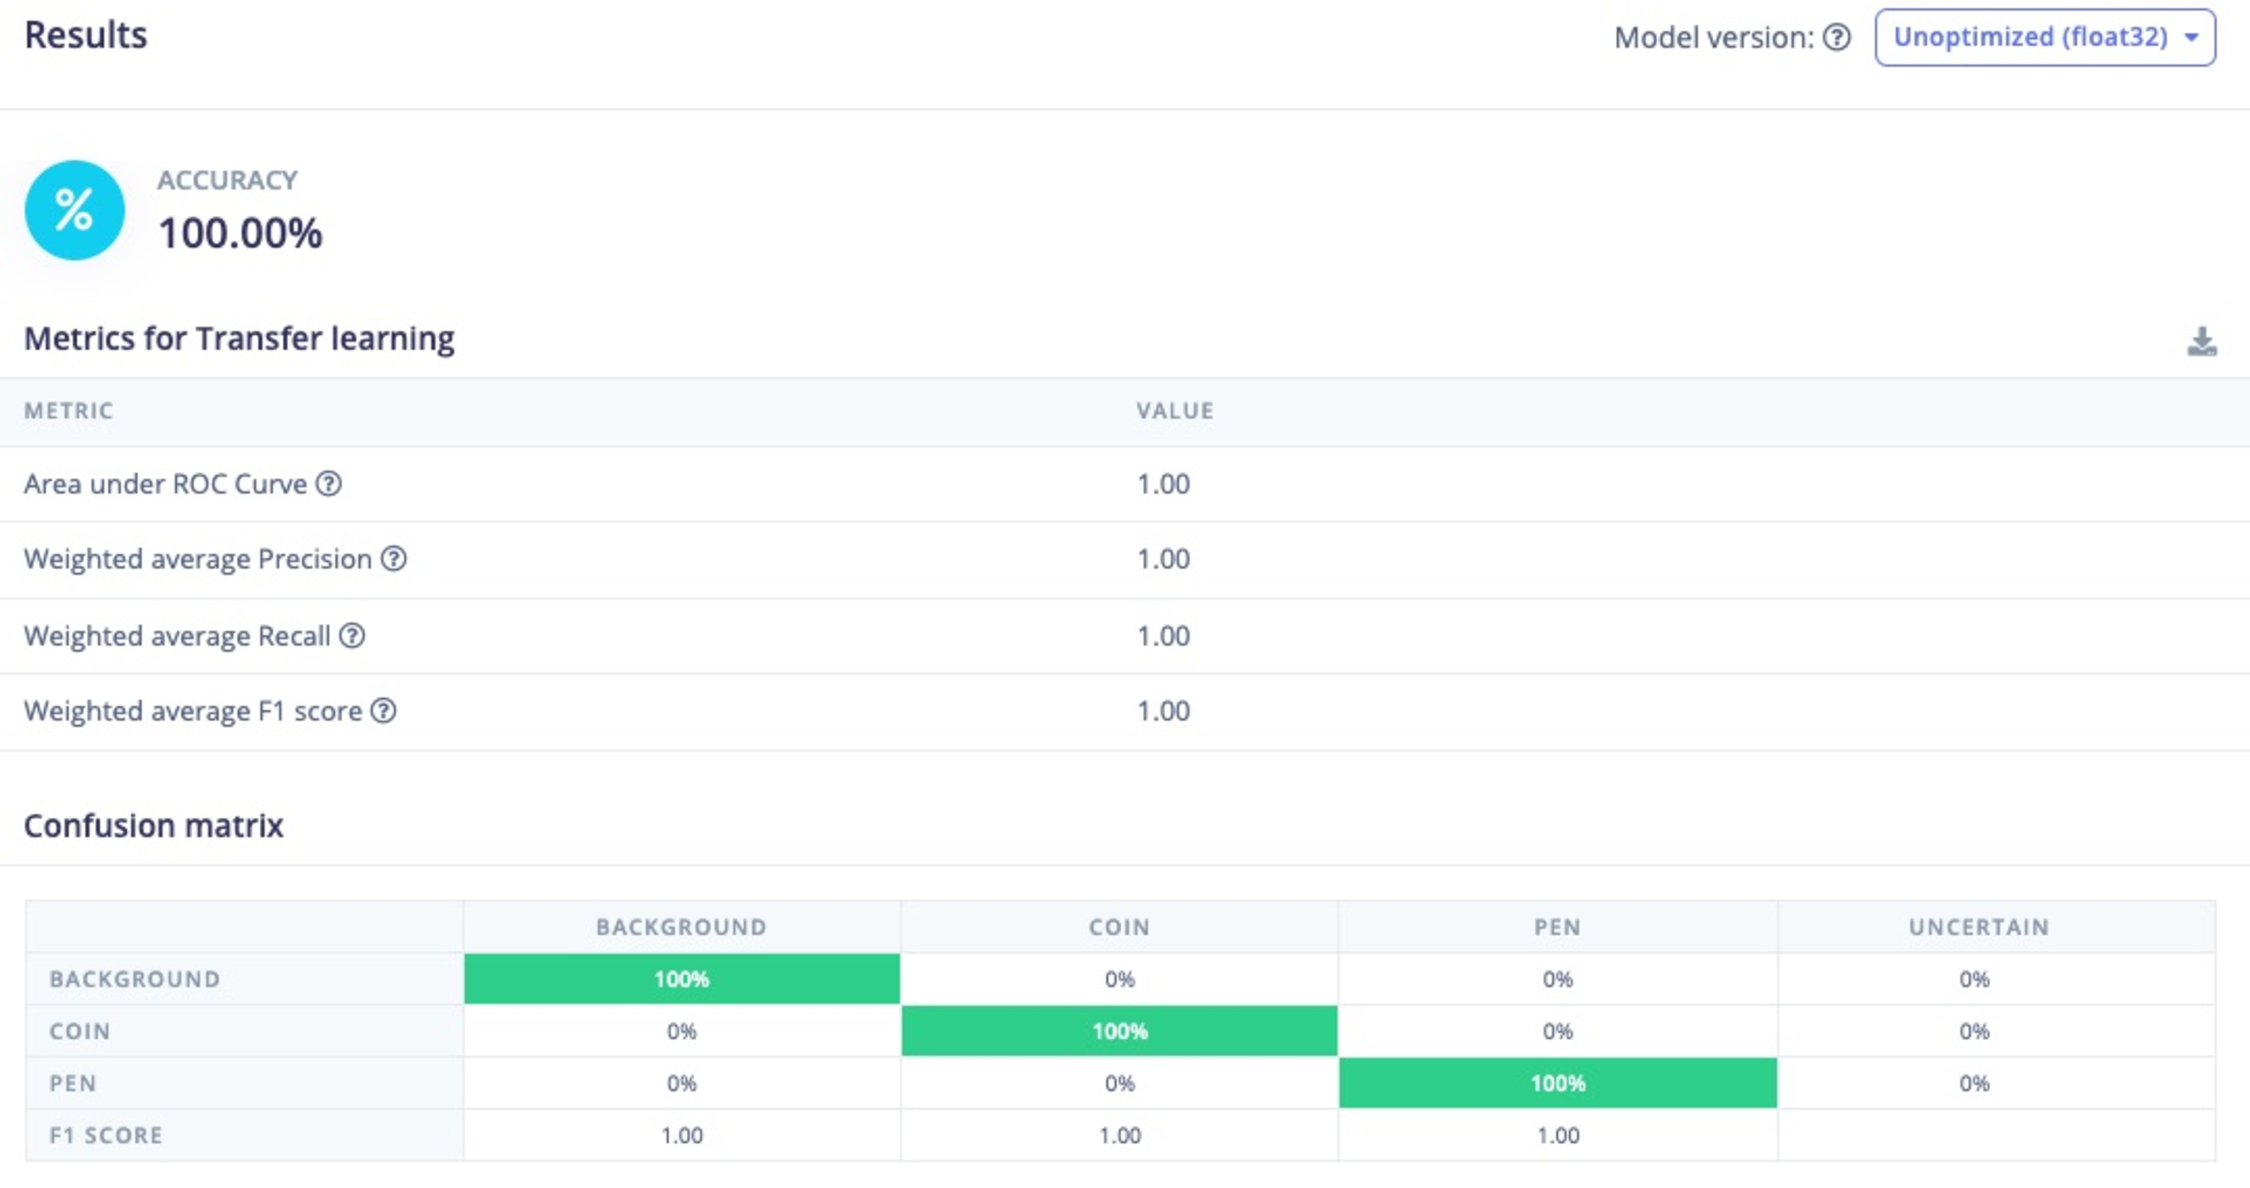
\includegraphics[width=0.8\linewidth]{Resources/Validation_results.pdf} % <-- replace with your filename
    \caption{Validation results}
\end{figure}

To test the model on your phone, you can scan the following QR code:

\begin{figure}[h!]
    \centering
    
\includegraphics[width=0.3\linewidth]{Resources/model_qr.pdf} % <-- replace with your filename
    \caption{EdgeImpulse model QR code}
\end{figure}